  \documentclass{mynotes}

%\geometry{showframe}% for debugging purposes -- displays the margins

\newcommand{\E}{\mbox{E}}
\newcommand{\MSE}{\mbox{MSE}}
\newcommand{\var}{\mbox{var}}


\usepackage{amsmath}
%\usepackage[garamond]{mathdesign}
\usepackage{url}

% Set up the images/graphics package
\usepackage{graphicx}
\setkeys{Gin}{width=\linewidth,totalheight=\textheight,keepaspectratio}
\graphicspath{{graphics/}}

\title[Exercises 6 $\cdot$ SSC 383D]{Exercises 7: Latent-feature models}
%\author[ ]{ }
\date{}  % if the \date{} command is left out, the current date will be used

% The following package makes prettier tables.  We're all about the bling!
\usepackage{booktabs}

% The units package provides nice, non-stacked fractions and better spacing
% for units.
\usepackage{units}

% The fancyvrb package lets us customize the formatting of verbatim
% environments.  We use a slightly smaller font.
\usepackage{fancyvrb}
\fvset{fontsize=\normalsize}

% Small sections of multiple columns
\usepackage{multicol}

% Provides paragraphs of dummy text
\usepackage{lipsum}

% These commands are used to pretty-print LaTeX commands
\newcommand{\doccmd}[1]{\texttt{\textbackslash#1}}% command name -- adds backslash automatically
\newcommand{\docopt}[1]{\ensuremath{\langle}\textrm{\textit{#1}}\ensuremath{\rangle}}% optional command argument
\newcommand{\docarg}[1]{\textrm{\textit{#1}}}% (required) command argument
\newenvironment{docspec}{\begin{quote}\noindent}{\end{quote}}% command specification environment
\newcommand{\docenv}[1]{\textsf{#1}}% environment name
\newcommand{\docpkg}[1]{\texttt{#1}}% package name
\newcommand{\doccls}[1]{\texttt{#1}}% document class name
\newcommand{\docclsopt}[1]{\texttt{#1}}% document class option name

\newcommand{\N}{\mbox{N}}
\newcommand{\thetahat}{\hat{\theta}}
\newcommand{\sigmahat}{\hat{\sigma}}
\newcommand{\betahat}{\hat{\beta}}


\begin{document}

\maketitle% this prints the handout title, author, and date


\section{Projecting downward}

A question one often encounters in statistics is: given a $p$-dimensional vector, how do we project it down into a smaller $k$-dimensional space in a way that preserves as much of the information in the original data as possible? The point is to represent a large amount of information in a tractable, more parsimonious way---in other words, to cut through the clutter.

You already know one way of doing this, namely linear regression.  Given an $n$-dimensional outcome vector $y$ and a matrix of covariates $X$, the fitted values $\hat{y} = X (X^T X)^{-1} X^T y$ (or their equivalents arising from a Bayesian model) involve a projection from $\mathcal{R}^n$ to $\mathcal{R}^p$.  But what if you don't have regressors $X$, only the outcomes $y$?

\subsection{A simple example: projection to $\mathcal{R}$}

Say we have $n$ observations of a $p$-dimensional outcome vector $y_i$. By $Y$, I mean the matrix whose $i$th row is the $i$th observation $y_i^T = (y_{i1}, \ldots, y_{ip})^T$.  (Remember our convention that vectors are column vectors.) Suppose for the moment that every column of $Y$ is standardized to have mean zero and unit variance.

Imagine projecting every observation $y_i$ into a one-dimensional subspace---that is, defining a new scalar outcome $z_i = y_i^T w_1$ for some vector $w_1$.  Presumably $w_1$ should be maximally information-preserving.  The question is how to operationalize this rather loose idea.

\begin{marginfigure}
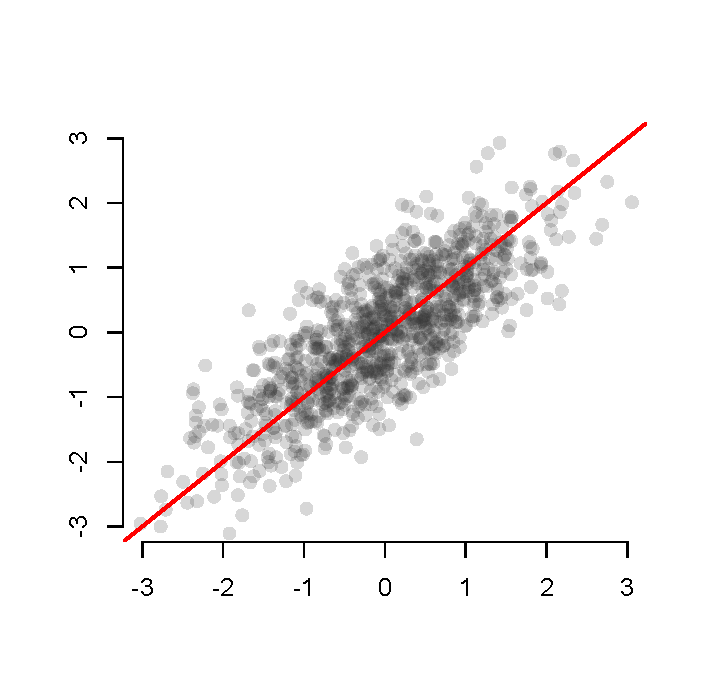
\includegraphics{cloud1.pdf}
\end{marginfigure}

Here's one way: choose $w_1$ so as to \textit{maximize the variance} of the projected values $z_i$.  The intuition for this is straightforward.  In the picture at right, the points can be described fairly well by projecting each one onto the diagonal line and reporting the single number $z_i$.  (Or equivalently, its actual position in $p$-dimensional space, which is $z_i w_1$---though this requires $p$ numbers.)  It's also easy to see that the projected points will have greater variance in this subspace than they would in any other choice of subspace.  Try drawing some other line through the point cloud; you'll see that the projections of the points onto this line would be more scrunched up than along the line I've drawn.

Mathematically, this means choosing $w_1$ such that the projected variance
$$
V_w = \frac{1}{n} \sum_{i=1}^n (z_i - \bar{z})^2 =  \frac{1}{n} \sum_{i=1}^n (y_i^T w_1 - \bar{z})^2
$$
is as large as possible.  Of course, we can blow up the variance to be as large as we want by choosing $w_1$ itself to be huge, so we must constrain it somehow.  A natural constraint is that $w_1$ is a unit vector: $w_1^T w_1 = 1$.

\begin{enumerate}

\item Characterize the relationship between the singular value decomposition of $Y$ and the eigenvalue decomposition of $\frac{1}{n} Y^T Y$.

\item Prove\footnote{Remember that the method of Lagrange multipliers is useful for optimizing under constraints.} that the unit-length $w_1$ which maximizes the projection variance is a right-singular vector of the data matrix $Y$ corresponding to the largest singular value $d_1$.  What is the relationship between $V_w$ and $d_1$?

\item Load the data in ``congress109.csv.''  The rows are members of the 109th U.S.~Congress; the columns are phrases uttered during floor speeches.  Entry $(i,j)$ in the matrix is the number of times member $i$ uttered phrase $j$.  Find the variance-maximizing one-dimensional projection, and compute the location of each member in this one-dimensional space.  (Meet R's built-in routines \verb|svd| and \verb|eigen|.) You've now moved from 1000 pieces of information about each member, to 1.  Consult the information in ``congress109members.csv.''  (You might find R's \verb|merge| command helpful.)  Does location in the  subspace you've defined seem to correlate with relevant political facts about each member?

\item Since each projected value is $z_i = y_i^T w_1$, we can write the whole column vector of $z_i$'s as $Z = Y w_1$, and the residuals from this projection as $R = Y - Z w_1^T$.  Each row of $R$ is the residual vector for the $i$th case, after the projection.

Now imagine applying the same procedure as above to the residuals: that is, finding the maximum-variance projection of each residual vector $r_i$, defined by some new vector $w_2$.  Prove that $w_2$ is the right-singular vector of the original data matrix $Y$ corresponding to the second largest singular value $d_2$.

Prove (by induction) that the $k$th principal component is the $k$th right-singular vector.  Here the $k$th principal component is defined to be the variance-maximizing projection of the residuals after subtracting the contributions to $Y$ of the first $k-1$ principal components.

\end{enumerate}

\newpage

\section{Factor models}

The principal-components representation of a $d$-dimensional data vector $y_i$ is
$$
y_i = \sum_{k=1}^d f_{i,k} w_k \, ,
$$
where $w_k$ is the $k$th principal component of the data matrix $Y$, and where $f_{i,k}$ is the projection of $y_i$ onto $w_k$.

The equation is of course exact if one uses all $d$ principal components.  But this involves keeping around the same amount of information as is required by the original data set---there is no summary or compression of the data, merely a re-expression of the data in the new coordinate system defined by the right-singular vectors of $Y$.

If we instead drop all but the first $c < d$ principal components, we can reconstruct the data approximately:
$$
y_i \approx \sum_{k=1}^c f_{i,k} w_k \, ,
$$
and by adding an error term, we restore precise equality:
$$
y_i =	 \sum_{k=1}^c f_{i,k} w_k  + \epsilon_i = W f_i + \epsilon_i \, .
$$
where $f_i$ is the $c$-vector of scores.  Presto: we have changed principal-component analysis into a \textit{factor model}, which involves explicit statistical assumptions about the errors $\epsilon_i$.   Each $f_i$ is the vector of \textit{factor scores} for observation $i$, while $W$ is called the loadings matrix, and is common to all observations.

Stacking up the whole system into a single matrix equation, we have
$$
Y^T = W F^T + E^T \, ,
$$
where $Y$ is the $n \times d$ matrix of observations, whose $i$th row is $y_i$; $W$ is the loadings matrix, and $F$ is the matrix whose $i$th row is $f_i$.  (If you find the transposes messy, simply switch the dimensions of $Y$ and $F$ and re-interprets rows as columns.)

If this looks like a family of related regressions, that's because it is---just one where both the responses and predictors are unknown!  We will require some identifying restrictions in order to estimate them both.

\begin{enumerate}

\item  We'll start with a Gaussian factor model. Suppose that $f_i \sim N(0, I)$, and that $\epsilon_i \sim N(0, \Psi)$ for some diagonal matrix $\Psi = \mbox{diag}(\psi_1, \ldots, \psi_d)$.  What does this imply about the distribution of $y_i$?

\item Suppose that each element of the factor-loadings matrix $w_{jk}$ is assigned a Gaussian prior, whose variance is $\tau^2_k$ (that is, a different variance for each column of the loadings matrix).  What is the conditional posterior distribution of $W_j$, the $j$th row of $W$?

\item What is the conditional posterior distribution for $f_i$, given the data and the loadings matrix $W$?

\item Suppose that $\psi_j \sim IG(1/2, 1/2)$ a priori.  What is its conditional posterior?

\item Code up a Gibbs sampler fot fitting a Gaussian factor model, for now assuming that $\tau^2_k$, the hyperparameter governing the variance of the elements in column $k$ of $W$, is large (effectively infinite).  Use your Gibbs sampler to estimate a three-factor model to the country-level monthly stock returns in ``CountryReturns.csv.''  Can you interpret the factors from your model?

\item If
$$
y_i =	 W f_i + \epsilon_i \, ,
$$
then we also have that
$$
y_i = W \Gamma^T \Gamma f_i + \epsilon_i
$$
as long as $\Gamma^T \Gamma = I$.  This suggests that the factors in your model are not uniquely identified: we could right-multiply the loadings matrix by $\Gamma^T$, so long as we right-multiply the factor scores by $\Gamma$.  This makes it hard to interpret the factors, since we could rotate them by an arbitrary orthogonal matrix of appropriate dimension.

Ponder this issue, and suggest a solution (or way to sidestep the problem) if one occurs to you.  We'll discuss in class!

\end{enumerate}

\end{document}

